\section{Installation}
\label{sec:installation}

\subsection{Windows 32 bits}

In order to successfully follow the examples in this manual and use
\emph{DSLTrans} you have to follow these steps carefully:

\subsubsection{Step 1}
Make sure you have java 1.6 or Java 1.7 installed. DSLTrans is not yet compatible with Java 1.8.

\subsubsection{Step 2}
Download and install SWI-Prolog version 5.10.2 (``w32pl5102.exe'') that is inside the \emph{DSLTrans-Release} folder in our repository:
\url{https://github.com/githubbrunob/DSLTransGIT}

\subsubsection{Step 3}
Download and extract Eclipse Modeling Tools, Luna Service Release 1.

\subsubsection{Step 4}
Set the environment variables shown in the figures \ref{fig:path_user}, \ref{fig:path_system} and \ref{fig:swi_pl_path} below.

\begin{figure}[h]
\begin{center}
  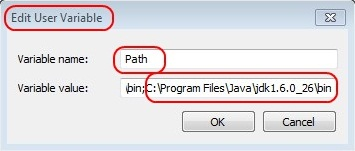
\includegraphics[scale=0.9]{imgs/path_user.jpg}
  \caption{Path to add to the \emph{user} \emph{Path} variable.}
  \label{fig:path_user}
\end{center}
\end{figure}

Note that, figure \ref{fig:path_user} you have to replace \verb=C:\Program Files\Java\jdk1.6.0_26\bin=
for your system's Java bin directory. Also, beware that the environment
variable you have to edit is the \emph{user} Path variable.

\begin{figure}[h]
\begin{center}
  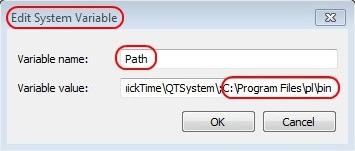
\includegraphics[scale=0.9]{imgs/path_system.jpg}
  \caption{Path to add to the \emph{system} \emph{Path} variable.}
  \label{fig:path_system}
\end{center}
\end{figure}

In figure \ref{fig:path_system}, you have to replace \verb=C:\Program Files\pl\bin= for your prolog installation
bin directory too. This time the variable to edit is the \emph{System} Path
variable.

\begin{figure}[h]
\begin{center}
  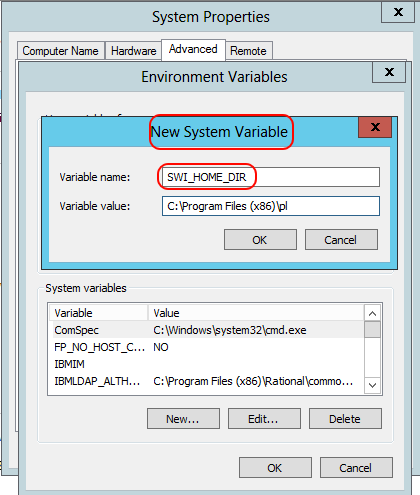
\includegraphics[width=0.6\textwidth]{imgs/swi_prolog_path.png}
  \caption{Path to add to the \emph{system} \emph{SWI\_HOME\_DIR} variable.}
  \label{fig:swi_pl_path}
\end{center}
\end{figure}

In figure \ref{fig:path_system}, you have to replace \verb=C:\Program Files (x86)\pl= for your prolog installation
directory.

\subsubsection{Step 5}

Now you have to copy the \verb=jpl.jar= file, in the 
\verb=C:\Program Files\pl\lib= 
directory, and paste it in Java's lib directory: 
\verb=C:\Program Files\Java\jdk1.6.0_26\lib=.

\begin{figure}[h]
\begin{center}
  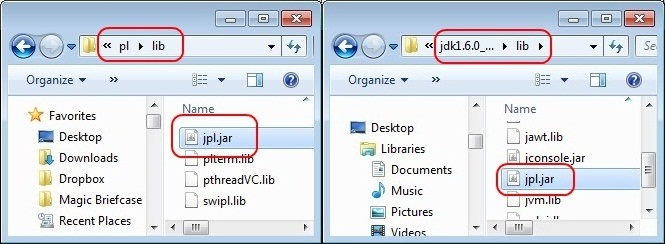
\includegraphics[width=0.8\textwidth]{imgs/jpl_cpy.jpg}
  \caption{Prolog's jpl.jar copied to Java's lib directory.}
  \label{fig:jpl_cpy}
\end{center}
\end{figure}

\subsubsection{Step 6}

Finally, you need to install the DSLTrans editor and transformer features from the Dsltrans update site.
For this you need to download and extract the DSLTransUpdateSite from the \emph{DSLTrans-Release} folder in our repository and install the features to eclipse using that update site.

\subsubsection{Step 7}

Afterwards, restart the pc.


\subsection{Windows 64 bits}

The installation of DSLTrans in Windows 64 bits is mostly similar to the installation of DSLTrans in Windows 32 bits except for the following steps.

\subsubsection{Step 2}

If you have Java 1.6 installed, download and install SWI-Prolog version 5.10.2 64 bits (``w64pl5102.exe'') that is inside the \emph{DSLTrans-Release} folder in our repository:
\url{https://github.com/githubbrunob/DSLTransGIT}

If you have Java 1.7 installed, download and install SWI-Prolog version 5.10.4 64 bits (``w64pl5102.exe'') that is inside the \emph{DSLTrans-Release} folder in our repository:
\url{https://github.com/githubbrunob/DSLTransGIT}

This distinction is necessary because prolog has a bug which causes access violations to JVM memory.
See section \ref{sec:faq} for details.



\clearpage


\begin{comment}	

Download & Install Prolog

Download & Install Plugins

Handle java library path

Path do admin com C:\Program Files\pl\bin

Copy jpl.jar to lib java folder

\end{comment}



% \subsection{Linux}
% TODO